\documentclass{beamer}

\usepackage[utf8]{inputenc}
\usepackage{hyperref}
\usepackage{lmodern}
\usetheme[style=light]{Nord}
\usefonttheme{professionalfonts}
\usepackage{amssymb, amsmath}
\usepackage [lambda,
advantage,
operators,
sets,
adversary,
landau,
probability,
notions,
logic,
ff,
mm,
primitives,
events,
complexity,
asymptotics,
keys]{ cryptocode }

\usepackage{amsfonts}

\usepackage[style=british]{csquotes}
\usepackage{graphicx}
\graphicspath{ {./img/} }

\usepackage{pgfplots}
    \pgfplotsset{
        compat=1.12,
    }

\def\signed #1{{\leavevmode\unskip\nobreak\hfil\penalty50\hskip1em
  \hbox{}\nobreak\hfill #1%
  \parfillskip=0pt \finalhyphendemerits=0 \endgraf}}

\newsavebox\mybox
\newenvironment{aquote}[1]
  {\savebox\mybox{#1}\begin{quote}\openautoquote\hspace*{-.7ex}}
  {\unskip\closeautoquote\vspace*{1mm}\signed{\usebox\mybox}\end{quote}}

\let\Tiny\tiny% http://tex.stackexchange.com/q/58087/5764
\newcommand{\disponslide}[2]{%
  \alt<#1>{#2}{\phantom{#2}}}

\newcommand{\overbar}[1]{\mkern 1.5mu\overline{\mkern-1.5mu#1\mkern-1.5mu}\mkern 1.5mu}

\newcommand{\plotcurveflexible}[4][thick, every plot/.style={smooth}]{
  % plot curve y^2 = x^3 + a x^2 + b x + c in range [-3,3]^2
  % parameter 1 (optional): style options for curve (color, etc)
  % parameter 2: curve parameter a
  % parameter 3: curve parameter b
  % paramater 4: curve paramter c
  \draw[gray] (-3,-3) rectangle (3,3);
  \draw[->,>=latex,gray] (-3,0) -- (3,0);
  \draw[->,>=latex,gray] (0,-3) -- (0,3);
  \draw[name path=curve, #1] plot[id=curve#2#3#4, raw gnuplot] function {
    f(x,y) = y**2 - x**3 -#2*x**2 - #3*x - #4;
    set xrange [-3:3];
    set yrange [-3:3];
    set view 0,0;
    set isosample 50,50;
    set cont base;
    set cntrparam levels incre 0,0.1,0;
    unset surface;
    splot f(x,y);
  };
}

\newcommand{\plotcurve}[3][thick, every plot/.style={smooth}]{
  % plot curve y^2 = x^3 + a x + b in range [-3,3]^2
  % parameter 1 (optional): style options for curve (color, etc)
  % parameter 2: curve parameter a
  % parameter 3: curve parameter b
  \draw[gray] (-3,-3) rectangle (3,3);
  \draw[->,>=latex,gray] (-3,0) -- (3,0);
  \draw[->,>=latex,gray] (0,-3) -- (0,3);
  \draw[name path=curve, #1] plot[id=curve#2#3, raw gnuplot] function {
    f(x,y) = y**2 - x**3 - #2*x - #3;
    set xrange [-3:3];
    set yrange [-3:3];
    set view 0,0;
    set isosample 50,50;
    set cont base;
    set cntrparam levels incre 0,0.1,0;
    unset surface;
    splot f(x,y);
  };
}

\usepackage{tikz}
\usetikzlibrary{arrows,positioning,intersections}

%Information to be included in the title page:
\title{Elliptic Curve Cryptography}
\subtitle{an introduction which is entirely too short}
\author{Giacomo Fenzi}
\institute{ETH Zurich}
\date{6 January 2022}



\begin{document}

\frame{\titlepage}

\begin{frame}
    \frametitle{Motivation}
    \begin{aquote}{Serge Lang}
    It is possible to write endlessly on elliptic curves. \\ (This is not a threat.)
    \end{aquote}
    \pause
    \begin{itemize}
        \item<2-> Elliptic curves are everywhere in cryptography
        \item<3-> Power $\approx 70\%$ of TLS Exchanges
        \item<4-> Coolest post quantum cryptography proposal
        \item<5-> Fascinating mathematically
    \end{itemize}
\end{frame}

\begin{frame}
    \frametitle{Outline}
    \begin{itemize}
        \item<1-> Historical Notes
        \item<2-> Mathematical Background 
        \item<3-> Addition on Elliptic Curves
        \item<4-> Discrete Logarithm and Diffie Hellman
        \item<5-> Pairings
        \item<6-> Isogenies
    \end{itemize}
\end{frame}
\section{History}

\begin{frame}
    \frametitle{Diophantine Equations}
    Historically originated in the context of solving Diophantine equations such as
    \[ X^n + Y^n = Z^n, \; \; X,Y,Z \in \ZZ \]
    \pause
    or equivalently
    \[ x^n + y^n = 1, \; \; x, y \in \QQ \]
    \pause
    Often very hard, and in general undecidable\footnote{In fact, already undecidable with 11 integers variables!}! 

    Let us see what we can do...

\end{frame}

\begin{frame}
    \frametitle{One variable}
    \[ a_n x^n + a_{n-1} x^{n-1} + \dots a_1 x + a = 0 \]
    \pause
    Quite easy! We can show that:
    \begin{theorem}
        Let $\frac{p}{q} \in \QQ$ be a solution of the above equation. 
        Then $q$ divides $a_n$ and $p$ divides $a_0$.
    \end{theorem}
    \pause
    Check the finite list of candidates.

    Alternatively, solve numerically and find candidate of form $\frac{b}{a_n}$
\end{frame}

\begin{frame}
    \frametitle{Linear and Quadratic}
    \[ a x + b y = c \]
    \pause
    \begin{theorem}
        Has infinitely many rational solution. If $\gcd(a, b)$ does not divide $c$, then no integers solutions.
        Else, infinitely many.
    \end{theorem}
    \pause
    \[ a x^2 + b x y + c y^2  + d x + e y + f = 0 \]
    \pause
    These are rational points on a conic. 
    \begin{itemize}
        \item Given a rational point, all of them can be found geometrically
        \item Hasse principle allows us to test if a rational point exists
    \end{itemize}

\end{frame}

\begin{frame}
    \frametitle{Cubics}
    What about:
    \[ a x^3 + b x^2 y + c x y^2 + d y^3 + e x^2 + f x y + g y^2 + h x + i y + j = 0 \; ? \]
    \pause
    This is the general form of an elliptic curve!
    \pause
    We have that 
    \begin{theorem}[Mordell]
        If the curve is non singular, and it has a rational point then the group of rational points is finitely generated
    \end{theorem}
    \pause
    But no equivalent of Hasse principle!
    \pause
    \begin{center}
        \textbf{Elliptic Curves $\neq$ Ellipse}
    \end{center}
\end{frame}

\section{Background}
\begin{frame}
    \frametitle{Fields}
    \begin{definition}
        A field $K$ is set together with two operations $+, \cdot$ such that 
        \begin{itemize}
            \item $K$ is an abelian group under $+$ with identity $0$
            \item $K - \{ 0 \}$ is an abelian group under multiplication with identity $1$.
            \item For every $a,b,c \in K$ we have that $a (b + c) = ab + ac$
            \item $0 \neq 1$
        \end{itemize}
    \end{definition}
    \pause
    Informally, we can add, subtract, multiply and divide non zero elements.
\end{frame}

\begin{frame}
    \frametitle{Finite Fields}
    We are mostly interested in finite fields.:
    \begin{theorem}
        For every prime $p$, and every $n \in \ZZ^+$ there is an unique field of size $p^n$, which we denote 
        by either $\mathbb{GF}(p^n)$ or $\FF_{p^n}$
    \end{theorem}
    \pause
    
    If $n = 1$, then $\FF_{p} = \ZZ_p$, if not we can write them as
    \[ \FF_{p^n} = \frac{\FF_{p}[X]}{(f(x))} \]
    where $f(x)$ is an irreducible polynomial of degree $n$.
\end{frame}

\begin{frame}
    \frametitle{Characteristic}
    For any field, $\mathrm{char}(\FF)$ is the least integer\footnote{Or $\infty$ if no such integer exists} $\ell$ such that 
    \[ \underbrace{1 + \dots 1}_{\ell \text{ times}} = 0 \]
    We have that $\mathrm{char}(\FF_{p^n}) = p$. 
\end{frame}

\begin{frame}
    \frametitle{Field Extensions}
    Let $k, K$ be two fields. If there is an homomorphism $k \to K$, we can identify $k$ with a subfield of $K$. 
    In that case, $K$ is a \textbf{field extension} of $k$ which we denote by $k \subseteq K$. 
    
    \pause
    Given any field $K$ we can construct the algebraic closure $\overbar{K}$ which is the smallest algebraically closed extension containing $K$.

    Some examples:
    \begin{itemize}
        \item<1-> $\QQ \subseteq \mathbb{R} \subseteq \mathbb{C}$
        \item<2-> $\FF_p \subseteq \FF_{p^2} \subseteq \FF_{p^3} \dots \subseteq \overline{\FF}_{p}$
    \end{itemize}
\end{frame}

\section{Elliptic Curves}
\subsection{Representation and Group Law}
\begin{frame}
    \frametitle{Weierstrass Form} 
    \begin{align*}
        a x^3 + b x^2 y + c x y^2 + d y^3 +& e x^2 + f x y + g y^2 + h x + i y + j = 0 \\
        &\disponslide{2-}{\big\downarrow} \\
        \disponslide{2-}{y^2 + a xy + b y} & \disponslide{2-}{= x^3 + c x^2 + d x + e} \\
        &\disponslide{3-}{\bigg\downarrow \; \mathrm{char}(K) \neq 2, 3} \\
        \disponslide{3-}{y^2 = x^3 }&\disponslide{3-}{+ a x + b}
    \end{align*}
    \onslide{4-}{Much easier to manage!}
\end{frame}

\begin{frame}
    \frametitle{Elliptic Curves}
    \begin{definition}
        Let $k$ be a field. An elliptic curve $E$ over $k$ (denoted by $E/k$) is given by 
        \[ E: y^2 = x^3 + a x + b \]
        for $a, b \in k$. 
        \pause
        For any extension $k\subseteq K$ we define
        \[ E(K) = \set{(x, y) \in K \times K \mid y^2 = x^3 + a x + b } \cup \set{ \infty } \]
    \end{definition}
    \pause
    Mathematicians are often interested with $E(\QQ) \subseteq E(\mathbb{R}) \subseteq E(\mathbb{C})$ but we mostly consider the finite case.
\end{frame}


\begin{frame}
    \frametitle{Elliptic curves}
    \begin{center}
        
    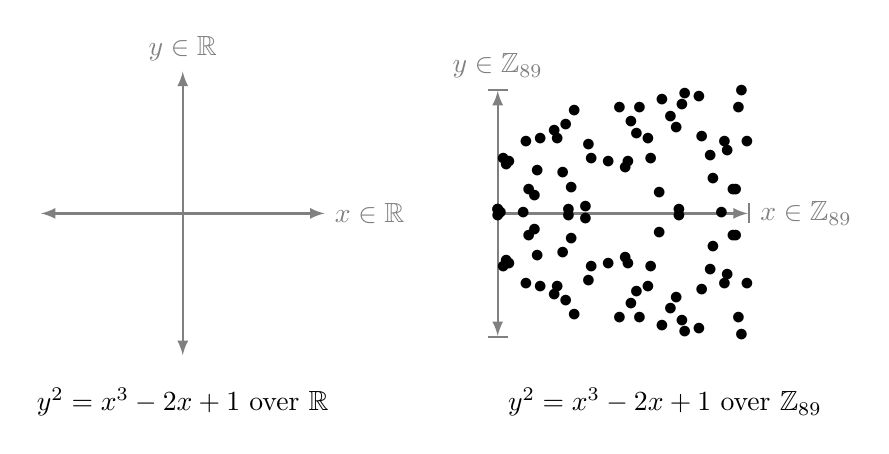
\begin{tikzpicture}[thick,>=latex,scale=0.8]
    % Curve over R

    % Requires GNUplot installation (part of TeXLive)
    \begin{scope}[scale=.75]
      \draw[<->,gray] (-3,0) -- (3,0) node[right] {$x \in \mathbb{R}$};
      \draw[<->,gray] (0,-3) -- (0,3) node[above] {$y \in \mathbb{R}$};
      \draw[thick, name path=curve, every plot/.style={smooth}] plot[id=curve-21, raw gnuplot] function {
        f(x,y) = y**2 - x**3 + 2*x - 1;
        set xrange [-3:3];
        set yrange [-3:3];
        set view 0,0;
        set isosample 50,50;
        set cont base;
        set cntrparam levels incre 0,0.1,0;
        unset surface;
        splot f(x,y);
      };

    \end{scope}

    \node at (0,-3) {$y^2 = x^3 - 2 x + 1$ over $\mathbb{R}$};
    
    \pause
    % Curve over Z_p

    % Generate list of points with Sage:
    % E = EllipticCurve(GF(89), [-2,1])
    % E.order()
    % print [(P[0],P[1]) for P in E]
    \begin{scope}[xshift=5cm, scale=.045]
      \draw[|<->|,gray] (0,-44) -- (0,44) node[above] {$y \in \mathbb{Z}_{89}$};
      \draw[->|,gray] (0,0) -- (89,0) node[right] {$x \in \mathbb{Z}_{89}$};
      \foreach \point in {
        (0, 1), (0, 1), (0, -1), (1, 0), (2, 19), (2, -19), (3, 17), (3, -17), (4, 18), (4, -18), (9, 0),
        (10, 25), (10, -25), (11, 8), (11, -8), (13, 6), (13, -6), (14, 15), (14, -15), (15, 26), (15, -26),
        (20, 29), (20, -29), (21, 26), (21, -26), (23, 14), (23, -14), (24, 31), (24, -31), (25, 1), (25, -1), (26, 9), (26, -9), (27, 36), (27, -36),
        (31, 2), (31, -2), (32, 24), (32, -24), (33, 19), (33, -19), (39, 18), (39, -18),
        (43, 37), (43, -37), (45, 16), (45, -16), (46, 18), (46, -18), (47, 32), (47, -32), (49, 28), (49, -28),
        (50, 37), (50, -37), (53, 26), (53, -26), (54, 19), (54, -19), (57, 7), (57, -7), (58, 40), (58, -40),
        (61, 34), (61, -34), (63, 30), (63, -30), (64, 1), (64, -1), (65, 38), (65, -38), (66, 42), (66, -42),
        (71, 41), (71, -41), (72, 27), (72, -27), (75, 20), (75, -20), (76, 12), (76, -12), (79, 0),
        (80, 25), (80, -25), (81, 22), (81, -22), (83, 8), (83, -8), (84, 8), (84, -8), (85, 37), (85, -37), (86, 43), (86, -43), (88, 25), (88, -25)
      } {\node at \point {$\bullet$};}
    \end{scope}

    \node[right] at (5,-3) {$y^2 = x^3 - 2 x + 1$ over $\mathbb{Z}_{89}$}; % order: 96

  \end{tikzpicture}
\end{center}
\end{frame}

\begin{frame}
    \frametitle{Some elliptic curves}
    \begin{center}

    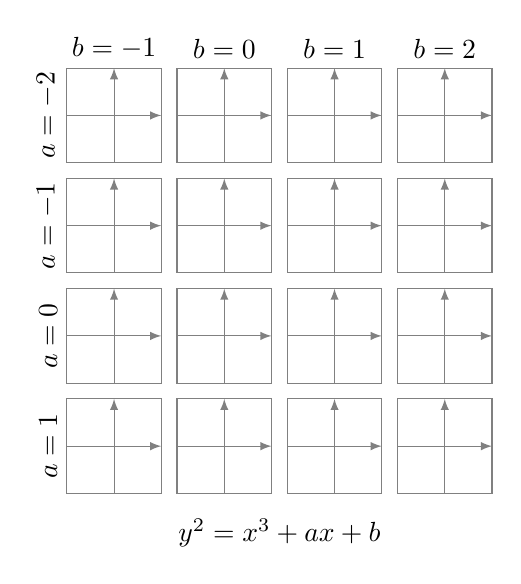
\begin{tikzpicture}[scale=0.8]
    \foreach \a in {-2,...,1} {
      \foreach \b in {-1,...,2} {
        \begin{scope}[xshift=1.75*\b cm,yshift=-1.75*\a cm,scale=.25]
          \plotcurve{\a}{\b}
        \end{scope}
      }
      \draw (-1.75*2+1,-1.75*\a) node[above,rotate=90] {$a=\a$};
    }
    \foreach \b in {-1,...,2} {
      \draw (1.75*\b,1.75*3-1) node[above] {$b=\b$};
    }
    \node[above] at (1.75/2,-2*1.75) {$y^2 = x^3 + a x + b$};
  \end{tikzpicture}
          
    \end{center}
\end{frame}
\begin{frame}
    \frametitle{More elliptic curves}
    \begin{center}

    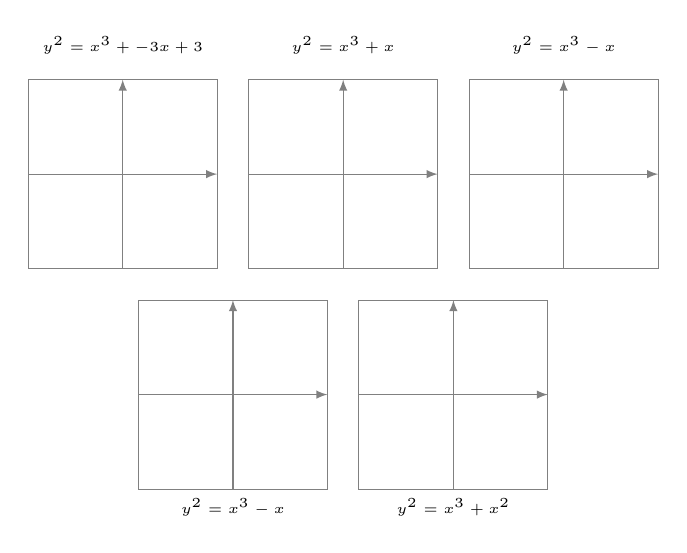
\begin{tikzpicture}[scale=0.8]
    
        \node[above] at (0,1.75) {\tiny $y^2 = x^3 + -3 x + 3$};
        \begin{scope}[xshift=0 cm,yshift=0 cm,scale=.50]
          \plotcurveflexible{0}{-3}{+3}
        \end{scope}
        \node[above] at (3.5,1.75) {\tiny $y^2 = x^3 + x$};
        \begin{scope}[xshift=3.5 cm,yshift=0 cm,scale=.50]
          \plotcurveflexible{0}{1}{0}
        \end{scope}
        \node[above] at (7,1.75) {\tiny $y^2 = x^3 - x$};
        \begin{scope}[xshift=7 cm,yshift=0 cm,scale=.50]
          \plotcurveflexible{0}{-1}{0}
        \end{scope}
        \node[below] at (1.75,-5) {\tiny $y^2 = x^3 - x$};
        \begin{scope}[xshift=1.75 cm,yshift=-3.5 cm,scale=.50]
          \plotcurveflexible{0}{0}{0}
        \end{scope}
        \node[below] at (5.25,-5) {\tiny $y^2 = x^3 + x^2$};
        \begin{scope}[xshift=5.25 cm,yshift=-3.5 cm,scale=.50]
          \plotcurveflexible{1}{0}{0}
        \end{scope}
  \end{tikzpicture}
          
    \end{center}
\end{frame}

\begin{frame}
    \frametitle{Discriminat}
    \begin{definition}
        Let $E: y^2 = x^3 + a x + b$ be an elliptic curve.

        The \textbf{discriminant} of $E$ is 
            \[ \Delta = -16 (4 a^3 + 27 b^2) \] 
        A curve is \textbf{singular} if $\Delta = 0$.
   \end{definition}
   \pause
    Alternatively, let $E: y^2 = f(x)$, and let $x_1, x_2, x_3$ be the roots of $f$. 
    \[ \Delta = (x_1 - x_2)^2(x_2 - x_3)^2(x_3 - x_1)^2 \]
    i.e. $\Delta = 0 \iff f$ has a repeated root.

    \pause
    From now on, all curves are assumed non singular.
    
\end{frame}

\begin{frame}
    \frametitle{$j$-invariant}
    \begin{definition}
         The $j$\textbf{-invariant} of $E$ is
            \[ j(E) = -1728 \frac{(4 A)^3}{\Delta} \]
    \end{definition} 
    \pause
    In fact, an isomorphism from a curve in short Weierstrass form must necessarily be:
    \[ (x, y) \mapsto (u^2 x, u^3 y) \]
    for $u \in \overbar{K}^*$ 
    \pause 
    and this yields:
     \begin{theorem}
        Let $E, E'$ be two elliptic curves over $K$. Then $E \cong E'$ over $\overbar{K}$ if and only if $j(E) = j(E')$. 
    \end{theorem}  
\end{frame}

\begin{frame}
    \frametitle{The Group Law} 
    \begin{center}
        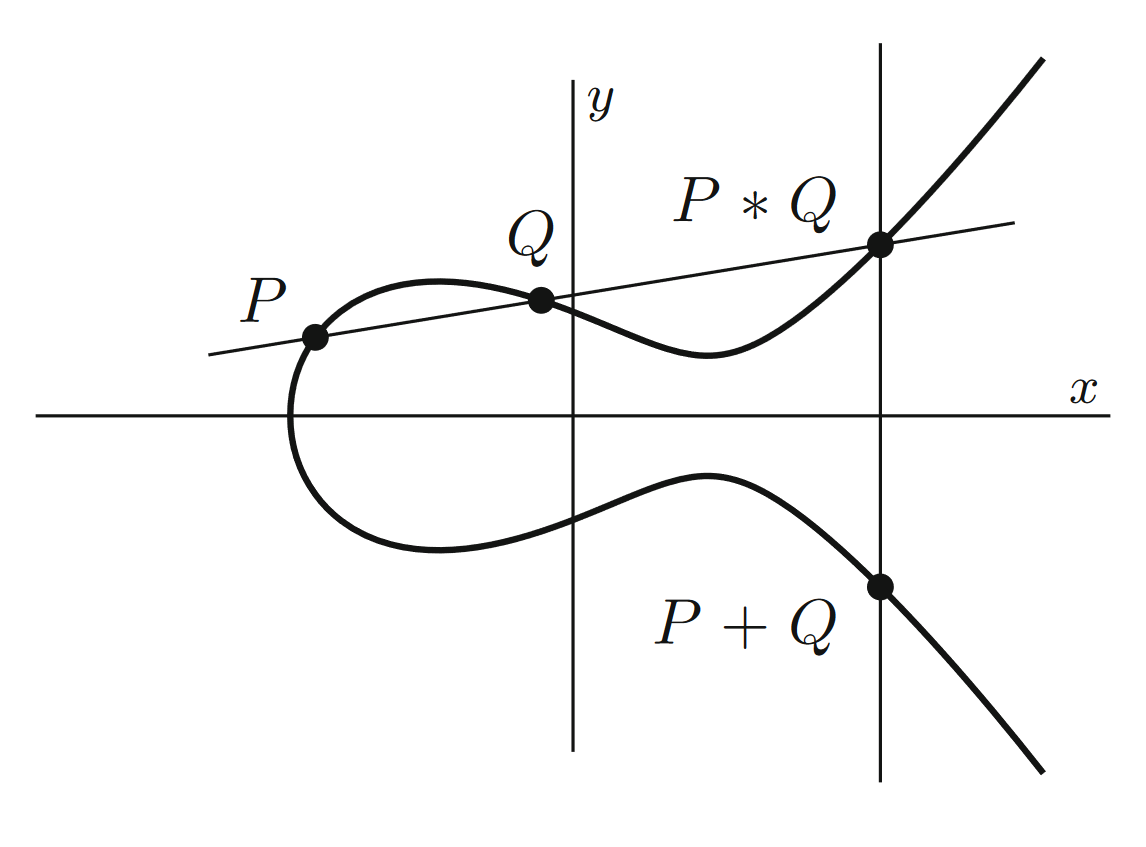
\includegraphics[width=20 em]{group_law.png}
    \end{center}
\end{frame}

\begin{frame}
    \frametitle{The Group Law: Formulae}
    Let $E: y^2 = x^3 + a x + b$ be an elliptic curve. Let $P_i = (x_i, y_i) \in E(K)$. 
    \pause
    Define 
    \[ -P_0 = (x_0, -y_0 )\]
    \pause
    Now, for $P_1 + P_2$: 
    \begin{itemize}
        \item<4-> If $x_1 = x_2$ and $y_1 = -y_2$, then $P_1 + P_2 = \infty$
        \item<5-> If $P_1 = \infty$ then $P_1 + P_2 = P_2$, and viceversa.
        \item<6-> Let $x_3 = \lambda^2 - x_1 - x_2$, $y_3 = \lambda(x_1 - x_3) - y_1$ where $\lambda$ is:
        \[ \lambda = \begin{cases}
            \frac{y_2 - y_1}{x_2 - x_1}, \; x_1 \neq x_2 \\
            \frac{3 x_1^2 + a}{2y_1},\; \text{otherwise}
        \end{cases} \]
    \end{itemize}
    \onslide<7->{
    This makes $E$ into an abelian group with identity $\infty$}
\end{frame}

\begin{frame}
    \frametitle{Scalar multiplication}
    For $n > 0, P \in E$ we write $[n]P = \underbrace{P + \dots + P}_{n \text{ times}}$. We then extend the notation by letting $[0]P = \infty$ and 
    $[-n]P = [n](-P)$. \\
    \pause

    We can compute $[n]P$ in $\Theta(\log n)$ group operations using double and add.
    
    \pause
    For $m \in \ZZ$ we define a map $[m]: E \to E$ accordingly, and write:
    \[ E[m] \coloneqq \ker[m] \]
    to be the $m$-\textbf{torsion subgroup} of $E$.
\end{frame}

\begin{frame}
    \frametitle{Number of Points on a curve}
    Heuristically, we expect $\approx q + 1$ points
    \pause
    \begin{theorem}[Hasse]
        Let $E$ be an elliptic curve defined over $\FF_q$.
        \[ \left|\#E(\FF_q) - q - 1\right| \leq 2 \sqrt{q} \] 
    \end{theorem}
    \pause
    Exact value can be efficiently found using Schoof's algorithm in $O((\log q)^8)$.
\end{frame}

\subsection{Discrete Log Crypto}

\begin{frame}
    \frametitle{Discrete Logarithm}
    Cryptography relies on hardness assumptions. 
    \pause
    \begin{definition}
        Let $\mathrm{Gen}(\secparam)$ be a p.p.t. algorithm that returns a group description $\GG = (+, P, q)$, where $\GG = \langle P \rangle$ and $q = \#\GG$.
        For an attacker $\adv$, define 
        \[\advantage{dlp}{\adv} = \Pr\left[\adv\left(\secparam, \GG, [k]P \right) = k \; \middle\vert \; \begin{matrix}
            \GG \sample \mathrm{Gen}(\secparam) \\
            k \sample \ZZ_q
        \end{matrix}
        \right] \]
        We say that the \textbf{discrete logarithm assumption} hold with respect to $\mathrm{Gen}$ if, for every p.p.t. attacker $\adv$, $\advantage{dlp}{\adv}[(\cdot)]$ is negligible.
    \end{definition}
\end{frame}

\begin{frame}
    \frametitle{Related Assumptions}
    In practice, we make stronger assumptions, such as Computational Diffie Hellman and Decisional Diffie Hellman. 
    \pause
    \begin{itemize}
        \item<2-> CHD: From $[x]P, [y]P$ compute $[xy]P$
        \item<3-> DDH: Distinguish $(P, [x]P, [y]P, [xy]P)$ from $(P, [x]P, [y]P, [z]P)$
    \end{itemize}
    \onslide<4->{
    Pairings make DDH easy on elliptic curves!}
    \onslide<5->{
    \[ \mathrm{DDH} \leq_R \mathrm{CDH} \leq_R\footnote{In fact equivalent in certain groups} \mathrm{DLP} \]}

    \onslide<6->{
    \textbf{Representation matters}! $\ZZ_{p-1} \cong \ZZ^*_p$ as groups but the discrete logarithm is trivial in the former, assumed hard in the latter. }
\end{frame}

\begin{frame}
    \frametitle{Why elliptic curves?}
    \pause
    \begin{center}
        \begin{tabular}{c c c c}
            Assumption & Group   & Best Algorithm & $\approx$ Complexity \\
            RSA        & $\ZZ_N$ & Number Field Sieve & $\mathrm{exp}(c ^3\sqrt{\log N})$ \\
            DLP        & $\FF^*_p$ & Number Field Sieve & $\mathrm{exp}(c ^3\sqrt{\log p})$ \\
            DLP        & $E(\FF_p)$ & Pollard Rho & $\sqrt{p}$ \\
        \end{tabular}
    \end{center}
    \pause
    \textbf{Best known attacks against ECC are generic attacks}
    \pause
    \begin{itemize}
        \item Shorter keysizes ($\approx 256$ vs\footnote{For 128 bits of security} 3072 bits)
        \item Faster computation\footnote{against other DLP schemes and private RSA ops}
    \end{itemize}
\end{frame}

\begin{frame}
    \frametitle{EC Diffie Hellman Key Exchange}
    Let $E$ be an elliptic curve over $\FF_q$. Let $p$ be a large prime dividing $\#E(\FF_q)$ and $P$ a point of order $p$. 
    \pause
    \procedureblock{Diffie Hellman}{
        \textbf{Alice} \> \> \textbf{Bob} \\
        x \sample \ZZ_q \> \> y \sample \ZZ_q \\
        Q_A = [x]P \> \> Q_B = [y]P \\
        \> \xrightarrow{Q_A} \> \\
        \> \xleftarrow{Q_B} \>  \\
        K = [x]Q_B \> \> K = [y]Q_A
    }
    \pause
    Correctness follows since:
    \[ K = [x]Q_B = [x][y]P = [xy]P = [y][x]P = [y]Q_A = K \]

\end{frame}

\begin{frame}
    \frametitle{Easy Elliptic Curves}
    \textbf{DLP is not equally hard on every curve}!
    \begin{itemize}
        \item<1-> Singular curves over $\FF_p$. Equivalent to DLP in\footnote{Or in some small extension} $\FF_p^*$ or $\FF_p^+$
        \item<2-> Curves and subgroups with small embedding degree. E.g. supersingular and anomalous curves
        \item<3-> Curves that admit pairings to small finite fields.
        \item<4-> Curves defined over $\FF_{p^k}$ for $k$ with small factors. GHS Method, Diem's Analysis.
    \end{itemize}
\end{frame}

\begin{frame}
    \frametitle{Pollard Rho}
    Collision search for $f: S \to S$. Let $x_0 \in S$, $x_n = f(x_{n-1})$.
    \pause
    Expected $\sqrt{\pi \#S/2}$ calls to $f$, constant memory.
    \pause
    \begin{center}
        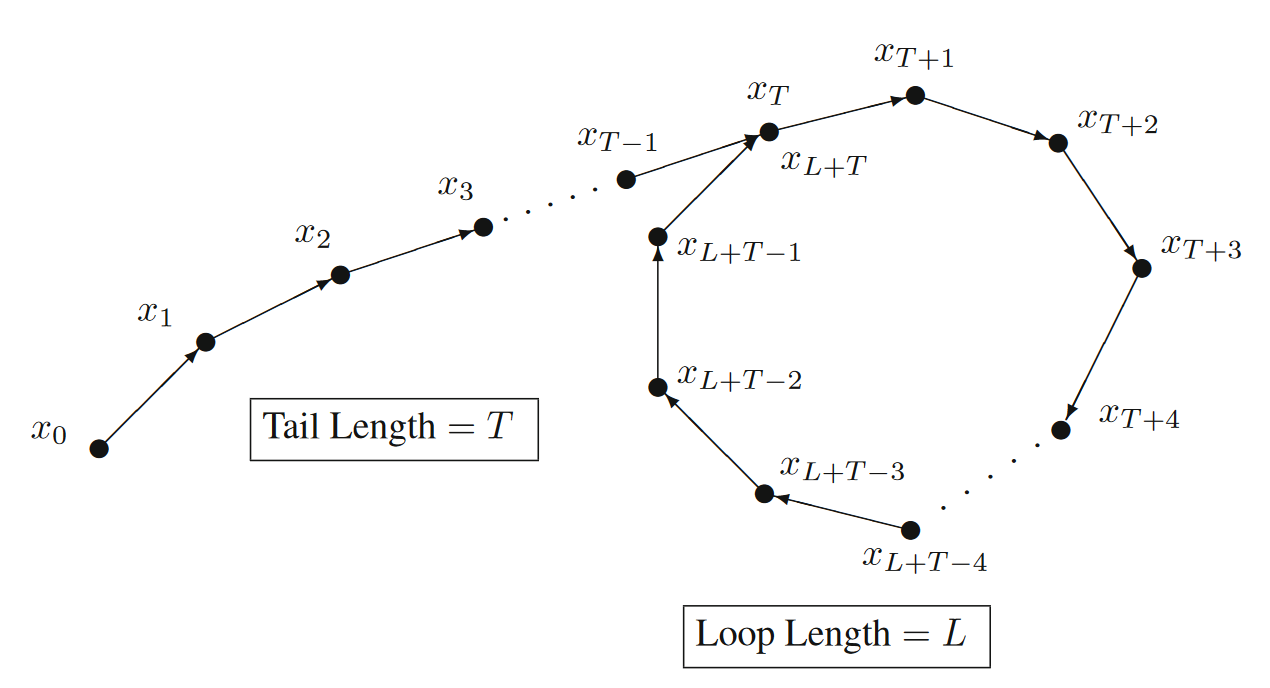
\includegraphics[width=25em]{pollard_rho.PNG}
    \end{center}
\end{frame}

\begin{frame}
    \frametitle{Pollard Rho}
    Let $G$ be a group of order $N$. We want to find $k$ s.t. $[k]P = Q$.
    \pause
    Split $G = A \sqcup B \sqcup C$ with $\# A \approx \# B \approx \#C$.
    \pause
    Define 
    \[ f(X) = \begin{cases}
        P + X, \; &X \in A \\
        [2]X, \; &X \in B \\
        Q + X, \; &X \in C
    \end{cases} \]
    \pause
    Let $X_0 = \infty$, then $X_i = [\alpha_i] P + [\beta_i] Q$ and we can track $\alpha_i, \beta_i$. 
    A collision $X_j = X_{j+\ell}$ with $\gcd(\beta_{j+\ell} - \beta_j, N) = 1$ allows us to solve the DLP with
    \[ k \equiv \frac{\alpha_j - \alpha_{j + \ell}}{\beta_{j+\ell} - \beta_j} \pmod{N} \]

\end{frame}

\subsection{Pairings}
\begin{frame}
    \frametitle{Pairings}
    \begin{definition}
        Let $\GG, \GG_T$ be two groups. A \textbf{pairing} is a map $e: \GG \times \GG \to \GG_T$ that is:
        \pause
        \begin{itemize}
            \item<2-> Non degenerate: 
            \[ e(S, T) = 1 \; \forall S \in \GG \implies T = 0_{\GG}  \]
            \item<3-> Bilinear:
            \[ e(S_1 + S_2, T) = e(S_1, T)e(S_2, T)\]
            \[ e(S, T_1 + T_2) = e(S, T_1)e(S_2, T_2)\]
            \item<4-> Alternating:
            \[ e(T, T) = 1 \]
            
        \end{itemize}
    \end{definition}
\end{frame}

\begin{frame}
    \frametitle{Weil Pairing}
    Every elliptic curve $E$ over $K$ admits an efficiently computable pairing
    \[ e_m : E[m] \times E[m] \to \mu_m \]
    where $\mu_m$ is the group of $m$-th root of unity. 

    \pause
    It is degenerate on cyclic subgroups of $E[m]$, so use modified Weil pairing
    \begin{align*}
        \langle \cdot , \cdot \rangle : E[m] &\times E[m] \to \mu_m \\
        \langle P, Q \rangle &= e_m(S, \phi(Q))
    \end{align*}
    For $\phi: E \to E$ a distorsion map\footnote{If it exists}

\end{frame}

\begin{frame}
    \frametitle{BLS Signatures}
    Let $\GG, \GG_T$ be cyclic groups of prime order $p$. Let $P$ be a generator of $\GG$, and $e$ a non degenerate pairing.
    Also, let $H: \bin^* \to \GG$
    \begin{center}
    \pause
    \begin{pcvstack}
        \begin{pchstack}
        \procedure{$\mathrm{Gen}(\secparam)$}{
            x \sample \ZZ_p \\
            pk \coloneqq [x]P \\
            sk \coloneqq x  \\
            \pcreturn (pk, sk)
        }
        \pause
        \procedure{$\mathrm{Sign}(sk, m)$}{
            Q \leftarrow H(m) \\
            \sigma \leftarrow [x]Q \\
            \pcreturn \sigma
        }
        \end{pchstack}

        \pause
        \procedure[space=auto]{$\mathrm{Verify}(pk, m, \sigma)$}{
            \pcreturn e(\sigma, P) =_? e(H(m), [x]P)
        }
    \end{pcvstack}
    \end{center}
    \pause
    Correctness by:
    \[ e(\sigma, P) = e([x]Q, P) = e(Q, P)^x = e(Q, [x]P) = e(H(m), [x]P) \]
 
\end{frame}

\subsection{Isogenies}
\begin{frame}
    \frametitle{Post Quantum}
    \begin{itemize}
        \item<1-> Discrete logarithms, RSA, and pairings broken by Shor's algorithm
        \item<2-> Can we recover?
        \item<3-> Yes, lattices, codes, multinear maps...
        \item<4-> \textbf{Isogenies!}
    \end{itemize}
\end{frame}

\begin{frame}
    \frametitle{Isogenies}
    ``Nice maps'' between elliptic curves.
    \pause
    \begin{definition}
        Let $E_1, E_2$ be elliptic curves. An \textbf{isogeny} is a morphism
        \[ \phi : E_1 \to E_2 \]
        with $\phi(\infty) = \infty$.
        If $\phi(E_1) \neq \set{\infty}$, $E_1$ is \textbf{isogenous} to $E_2$.
    \end{definition}
    \pause
    For example, the curves $y^2 = x^3 + x$ and $y^2 = x^3 - 3x + 3$ are isogenous over $\FF_{71}$ via the isogeny 
    \[ (x, y) \mapsto \left(\frac{x^3 - 4 x^2 + 30 x -12}{(x - 2)^2}, y\cdot\frac{x^3 - 6x^2 -14x + 35}{(x - 2)^3} \right)\]
\end{frame}

\begin{frame}
    \frametitle{Properties of isogenies}

    \begin{itemize}
        \item<1-> Each isogeny is also a group homomorphism
        \item<2-> The map $[m]: E \to E$ is an isogeny
        \item<3-> You can compose isogenies
        \item<4-> Each isogeny has a degree, and it is multiplicative $\deg(\phi \circ \psi) = \deg(\phi)\deg(\psi)$
        \item<5-> Each isogeny $\phi: E_1 \to E_2$ has a unique dual $\hat{\phi}: E_2 \to E_1$ such that 
        \[ \phi \circ \hat{\phi} = [\deg(\phi)] \]
        \item<6-> An isogeny between two Weierstrass curves has the form
        \[ (x, y) \mapsto \left(\frac{f}{h^2}(x), y\cdot \frac{g}{h^3}(x) \right) \]
    \end{itemize}
\end{frame}

\begin{frame}
    \frametitle{Separable and Inseparable Isogenies}
    \begin{definition}
        Let $E/k: y^2 = x^3 + ax + b$, with $\mathrm{char}(k) = p$. Define $E^{(p^r)}: y^2 = x^3 + a^{p^r} x + b^{p^r}$.
        The map:
        \[ \pi: E \to E^{(p^r)}, (x, y) \mapsto \left(x^{p^r}, y^{p^r} \right) \]
        is the $(p^r)$-\textbf{Frobenius isogeny}. 
        \pause 
        Note if $k = \FF_{p^r}$ then $E^{(p^r)} = E$
    \end{definition}
    \pause
    If an isogeny factors trough a Frobenius isogeny it is inseparable. 
    If it is a Frobenius followed by an isomorphisms, it is purely inseparable.
    \pause
    We are mostly  concerned with the separable case.

\end{frame}

\begin{frame}
    \frametitle{Kernel and Velu}
    \begin{theorem}
       There is a one to one correspondence between finite subgroups of elliptic curves 
       and separable isogenies from that curve, up to post-compostion with isomorphisms
       \pause
       \[ \text{kernels} \longleftrightarrow \text{isogenies} \]

    \end{theorem}
    \pause
       Let $E/k$, with $k$ a finite field. For any subgroup $H \leq E$ we can find an 
       isogeny with kernel $H$ in $\Theta(\#H)$ using Velu's formulas. We denote the target of 
       that isogeny by $E/H$
    
\end{frame}

\begin{frame}
    \frametitle{Computing large degree isogenies}
    \begin{itemize}
        \item<1-> Velu's formula are too slow for large degree
        \item<2-> Decompose $\ell^k$ isogenies in $k$ $\ell$-isogenies
        \item<3-> Speedup from $\Theta(\ell^k)$ to $\Theta(k^2 \ell)$
    \end{itemize}
    \onslide{4-}{
    Take $H \cong \ZZ_{\ell^k}$. Set $\ker \psi_i = [\ell^{k - i}](\psi_{i-1} \circ \dots \circ \psi_1)(H)$. 
    Then $\mathrm{deg}(\psi_i) = \ell$ and 

    \begin{center}
        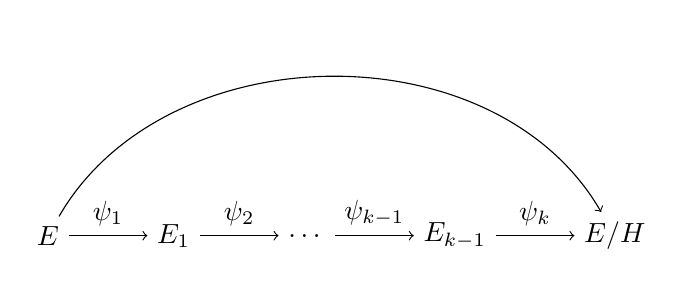
\begin{tikzpicture}
  \node (e) {$E$};
  \node (e1) [right=1 of e] {$E_1$};
  \node (dots) [right=1 of e1] {$\dots$};
  \node (ek1) [right=1 of dots] {$E_{k-1}$};
  \node (ek) [right=1 of ek1] {$E/H$};
  \draw[->] (e) to node [above] {$\psi_1$} (e1);
  \draw[->] (e1) to node [above] {$\psi_2$} (dots);
  \draw[->] (dots) to node [above] {$\psi_{k-1}$} (ek1);
  \draw[->] (ek1) to node [above] {$\psi_k$} (ek);
  \draw [->] (e) to [out=60,in=120]  (ek);
            
        \end{tikzpicture}
    \end{center}
    }

\end{frame}

\begin{frame}
    \frametitle{Supersingular Curves}
    \begin{definition}
        A curve $E$ defined over $K$ with $\mathrm{char}(K) = p$ is \textbf{supersingular}
        if $[p]$ is purely inseparable and $j(E) \in \FF_{p^2}$. 
        A curve that is not supersingular is \textbf{ordinary}
    \end{definition}
    \pause
    \begin{itemize}
        \item<2-> Something something order in a quaternion algebra?
        \item<3-> There are $\approx \lfloor \frac{p}{12} \rfloor$ supersingular curves over $\FF_{p^n}$.
        \item<4-> A supersingular curve has $p + 1$ points.
        \item<5-> Insecure for DLP
        \item<6-> Secure for CSSI (later)!
    \end{itemize}
    

\end{frame}

\begin{frame}
    \frametitle{Isogeny Problems}
    It is easy to find out if two curves are isogenous
    \pause
    \begin{theorem}
        Two curves $E_1, E_2$ over a finite field $k$ are isogenous over $k$ if and only if $\#E_1(k) = \#E_2(k)$.
    \end{theorem}
    \pause
   Finding the isogeny is dramatically harder:
   \pause
   \begin{definition}
       The \textbf{computational supersingular isogeny problem} is as follows:
       Given two supersingular elliptic curves $E, E'$, find an isogeny between them. 
   \end{definition}
\end{frame}

\begin{frame}
    \frametitle{Isogeny Graphs}
    Look something like this! We focus on the second
    \begin{center}
        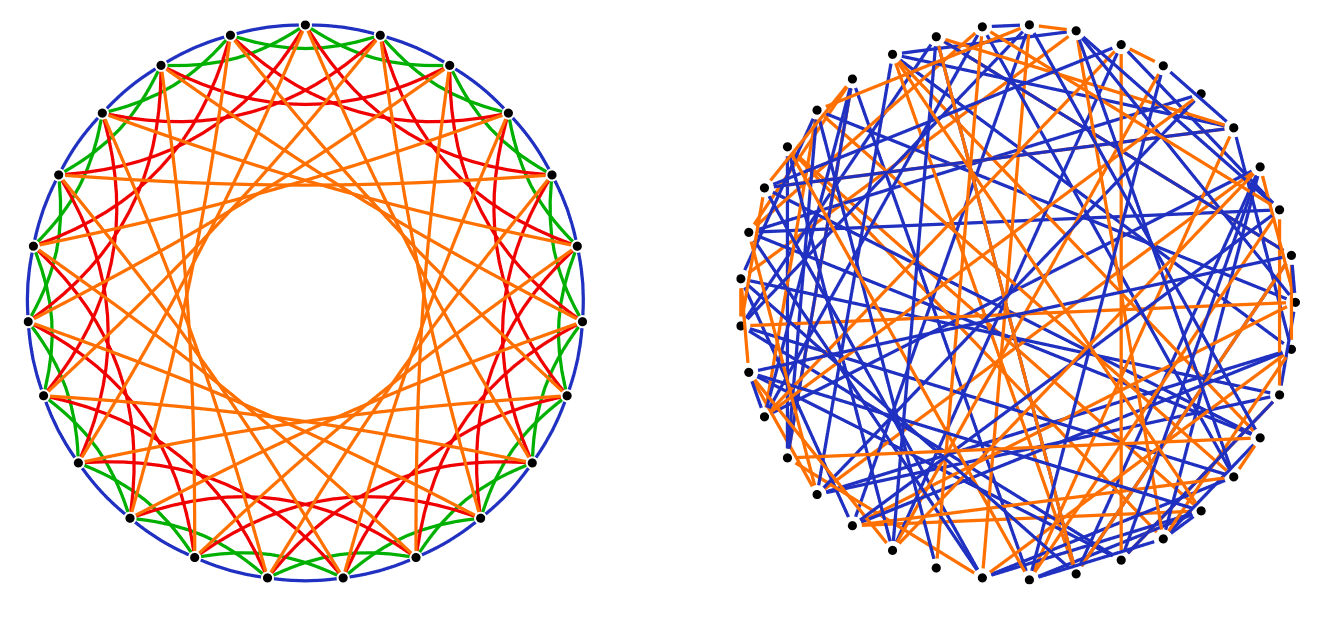
\includegraphics[width=28em]{isogeny_graph.PNG}
    \end{center}
\end{frame}

\begin{frame}
    \frametitle{Isogeny Graphs}
    Let $p, \ell$ be a primes.
    \pause
    \begin{definition}
        The $\ell$\textbf{-supersingular isogeny graph} has as:
        \begin{itemize}
            \item<2-> Vertices: Supersingular Elliptic curves over $\overline{\FF}_p$
            \item<3-> Edges: Separable isogenies from $E \to E'$
        \end{itemize}
        \onslide{4-}{
        Both up to isomorphisms (i.e. vertices are $j$-invariants)}
    \end{definition}
    \begin{itemize}
        \item<5-> We can represent vertices as elements of $\FF_{p^2}$
        \item<6-> Graph is directed
        \item<7-> Graph has good mixing properties
        \item<8-> Can walk in the graph with Velu's method
        \item<9-> Most vertices have degree $\ell + 1$
    \end{itemize} 

\end{frame}

\begin{frame}
    \frametitle{SIDH ($p = 2^4 3^3 - 1$)}
    \framesubtitle{Alice's pk}
    \begin{center}
        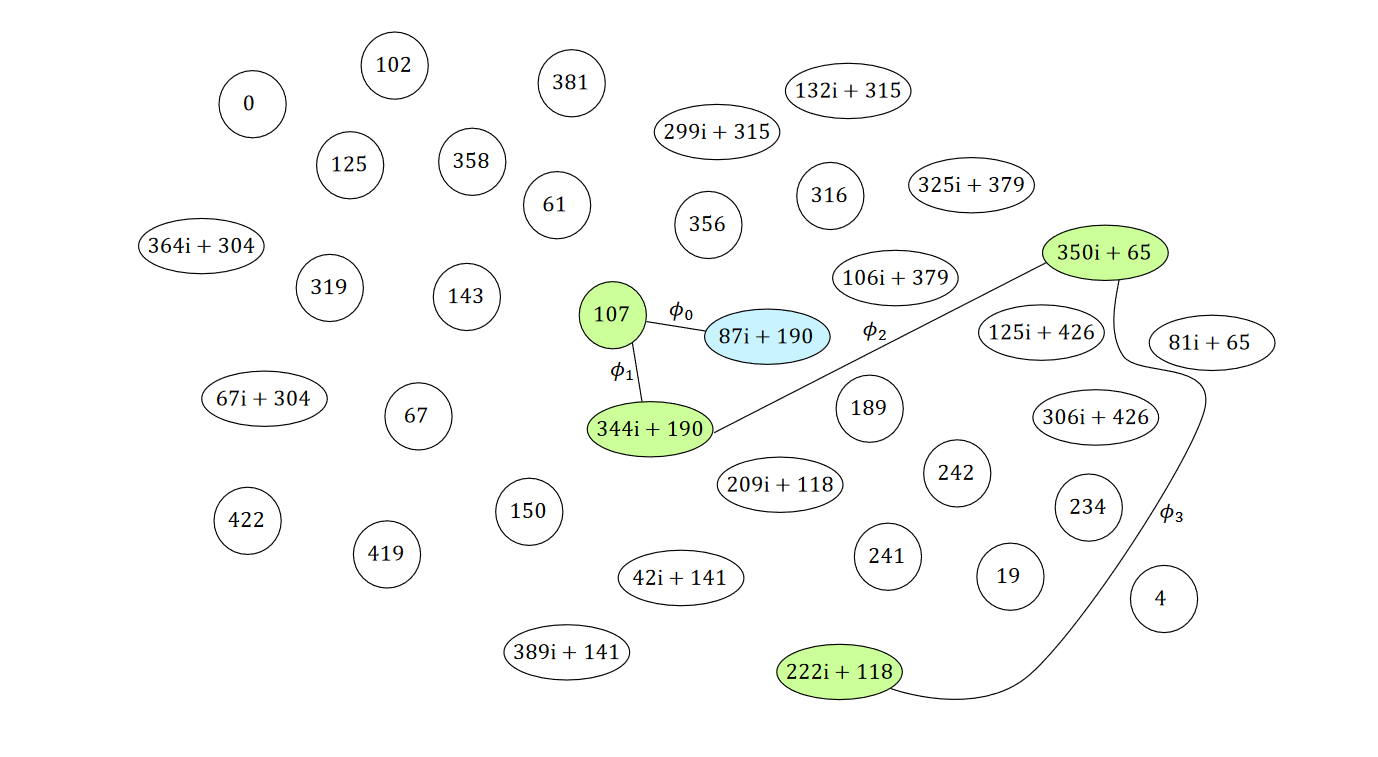
\includegraphics[width=25em]{alice_pk.PNG}
    \end{center}
\end{frame}

\begin{frame}
    \frametitle{SIDH ($p = 2^4 3^3 - 1$)}
    \framesubtitle{Bob's pk}
    \begin{center}
        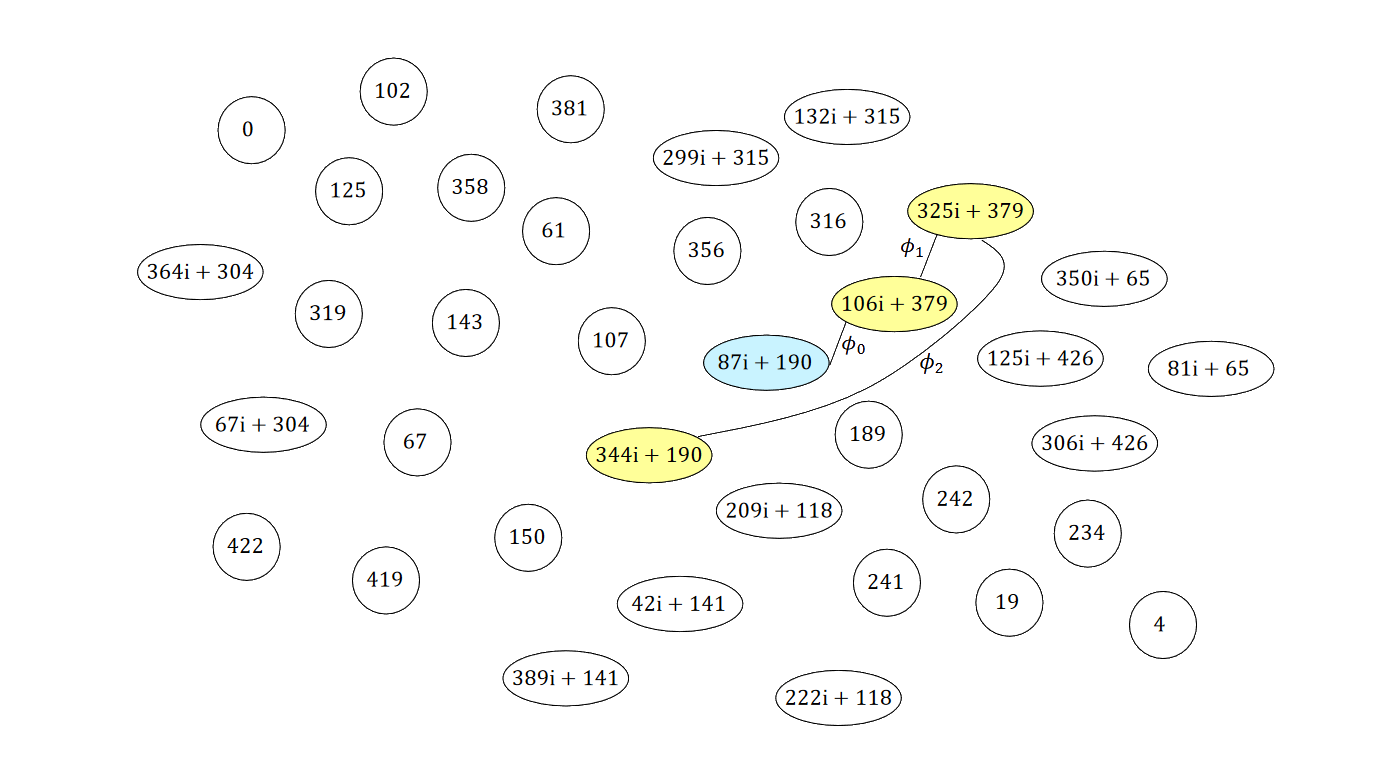
\includegraphics[width=25em]{bob_pk.PNG}
    \end{center}
\end{frame}

\begin{frame}
    \frametitle{SIDH ($p = 2^4 3^3 - 1$)}
    \framesubtitle{Alice's pk}
    \begin{center}
        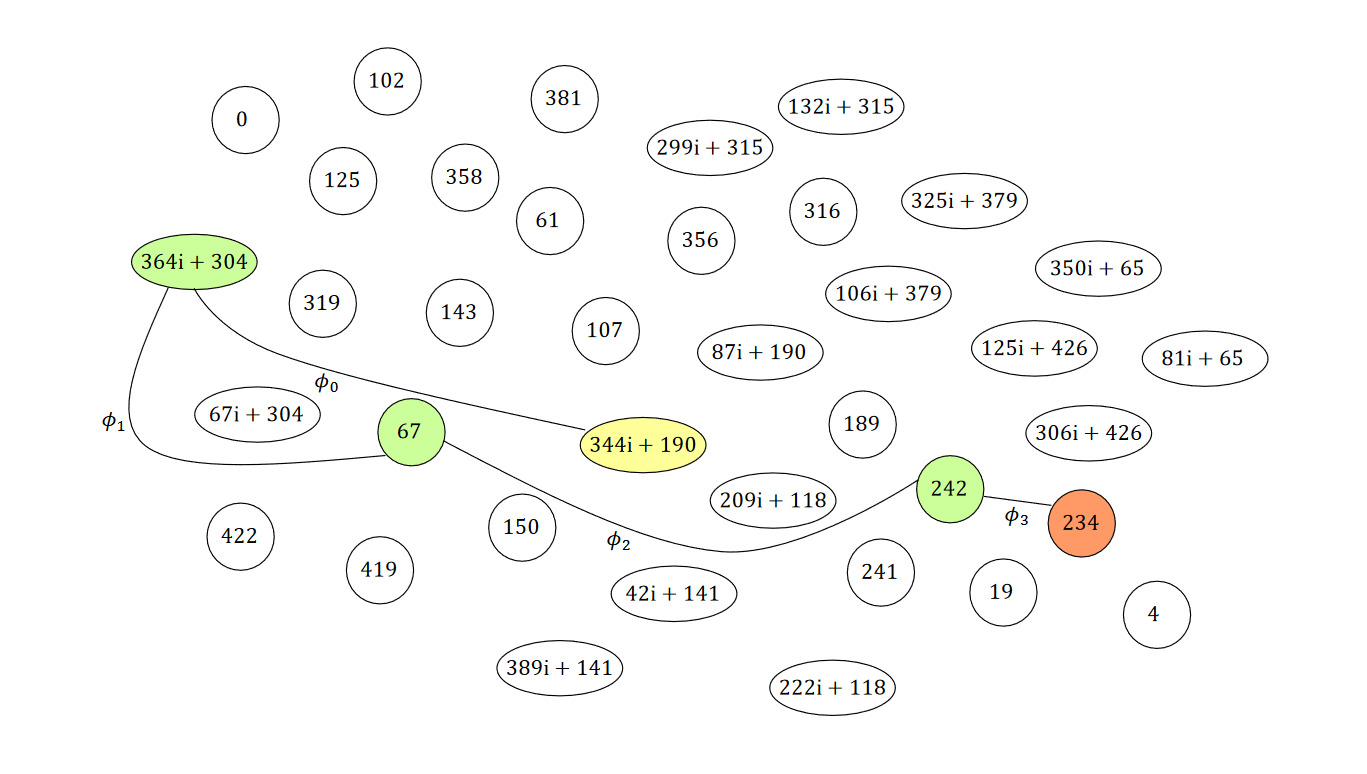
\includegraphics[width=25em]{alice_shared.PNG}
    \end{center}
\end{frame}

\begin{frame}
    \frametitle{SIDH ($p = 2^4 3^3 - 1$)}
    \framesubtitle{Alice's pk}
    \begin{center}
        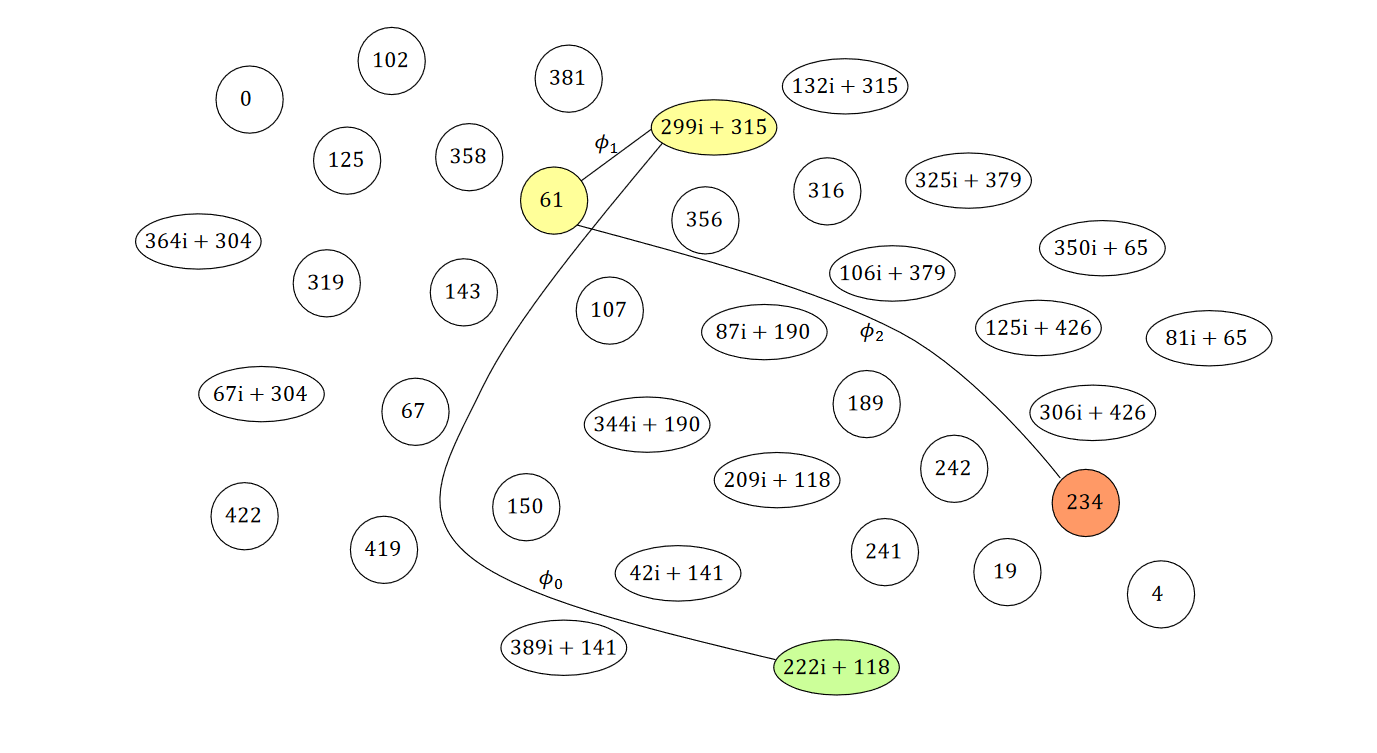
\includegraphics[width=25em]{bob_shared.PNG}
    \end{center}
\end{frame}

\begin{frame}
    \frametitle{SIDH}
    Picture to keep in mind:
\begin{center}
    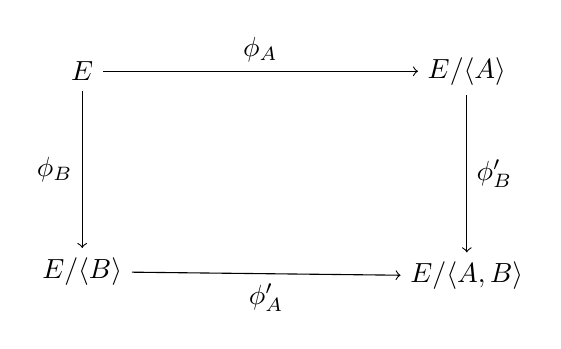
\begin{tikzpicture}
  \node (e) {$E$};
  \node (ea) [right=4 of e] {$E/\langle A \rangle$};
  \node (eb) [below=2 of e] {$E/\langle B \rangle$};
  \node (eab) [below=2 of ea] {$E/\langle A, B \rangle$};
  \draw[->] (e) to node [above] {$\phi_A$} (ea);
  \draw[->] (e) to node [left] {$\phi_B$} (eb);
  \draw[->] (ea) to node [right] {$\phi'_B$} (eab);
  \draw[->] (eb) to node [below] {$\phi'_A$} (eab);
\end{tikzpicture}
\end{center}
Details will follow
\end{frame}

\begin{frame}
    \frametitle{SIDH}
    Parties select $p = 2^{e_A} 3^{e_B} - 1$ prime,
    \pause a supersingular starting curve $E/\overline{\FF}_{p^2}$,
    \pause four points $P_A, P_B, Q_A, Q_B$ s.t.
    $\langle P_A, Q_A \rangle = E[2^{e_A}], \langle P_B, Q_B \rangle = E[3^{e_B}]$.
    \begin{itemize}
        \item<3-> Alice, Bob sample $n_A \sample \ZZ_{2^{e_A}}, n_B \sample \ZZ_{3^{e_B}}$, and compute $S_{X} = P_X + [n_X]Q_X$
        \item<4-> Alice computes the $2^{e_A}$ isogeny $\phi_A: E \to E/\langle S_A\rangle = E_A$
        \item<5-> Bob computes the $3^{e_B}$ isogeny $\phi_B: E \to E/\langle S_B\rangle = E_B$
        \item<6-> The public keys are $\mathrm{pk}_X = \left(E_X, P_X' = \phi_X(P_X), Q_X' = \phi_X(Q_X)\right)$
        \item<7-> Alice computes $S'_A = P'_B + [n_A] Q'_B$, and an isogeny $\phi'_A : E_B \to E/\langle S'_A \rangle = E_{AB}$
        \item<8-> Bob computes $S'_B = P'_A + [n_B] Q'_A$, and an isogeny $\phi'_B : E_A \to E/\langle S'_B \rangle = E_{BA}$
        \item<9-> The final secret is $j(E_{AB}) = j(E_{BA})$
    \end{itemize}
\end{frame}

\begin{frame}
    \frametitle{SIDH and SIKE}
    \begin{itemize}
        \item<1-> SIDH is vulnerable to active attacks
        \item<2-> SIKE uses the Fujisaki-Okamoto transform to fix this 
        \item<2-> SIKE in the Alternate Candidates of Round 3 of the NIST PQC competion
        \item<3-> Very short keys
        \item<3-> Currently a bit on the slow side
        \item<4-> Best known attack is classical
    \end{itemize} 
\end{frame}

\begin{frame}
    \frametitle{Security}
    Best attack is on CSSI problem.
    \pause 
    Suppose we want to find an $\ell^a$-isogeny  between $E_0 \to E_1$, both 
    supersingular over $\overbar{\FF}_p$.
    \pause Let $k \approx a/2$ and
    \begin{align*}
        S_{i, k} &\coloneqq \set{ H \leq E_i[\ell^k] \mid \; H \text{ cyclic}, |H| = \ell^k } \\
        S &\coloneqq \left( \set{0} \times S_{0, k} \right) \sqcup \left( \set{1} \times S_{1, k} \right) \\
        g: S &\to \FF_{p^2}, \; (i, H) \mapsto j(E_{i}/H)
    \end{align*}
    \pause
    A collision $g(0, H) = g(1, H')$ will solve CSSI.
    \pause To enable Pollard-Rho style methods, let $h: \FF_{p^2} \to S$ 
    be a hash function, and let:
    \[ f: S \to S,\; f \coloneqq h \circ g \]
\end{frame}

\begin{frame}
    \frametitle{Security}
    $h$ maps a set $\approx p/12$ to $S$ which has size $\approx p^{1/4}$ so introduces a lot of collisions.
    \pause
    To find a `golden' one we use the van Oorschot Wiener (vOW) algorithm. 
    \pause
    When using $m$ processors and $w$ memory cells, time complexity\footnote{In terms of $\ell^k$-isogeny computations} is 
    \[ \frac{2.5}{m}\sqrt{\#S^3/w} = O(p^{3/8})  \]
\end{frame}

\section{Conclusion}
\begin{frame}
    \frametitle{Conclusion}
    \begin{itemize}
        \item<1-> Elliptic curves are pretty damn cool
        \item<1-> We only scratched the surface!
        \item<2-> ECDH base of most of the web's key exchanges
        \item<3-> BLS Pairing based signatures both efficient and secure
        \item<4-> SIKE leverages isogenies for post quantum security
    \end{itemize}
    

\end{frame}

\section{Resources}

\begin{frame}[noframenumbering]
    \frametitle{Resources}
    \begin{itemize}
        \item [0]  J.H. Silverman, J.T. Tate, Rational Points on Elliptic Curves 
        \item [1].H. Silverman, The Arithmetic of Elliptic Curves\footnote{The bible}
        \item [2] D.A. Cox, Primes of the form $x^2 + n y^2$
        \item [3,4] L. Panny, notes: \href{https://yx7.cc/docs/misc/isog_bristol_notes.pdf}{[intro]} \href{https://yx7.cc/docs/misc/isogprob_bristol_notes.pdf}{[isogenies problems]}
        \item [5]C. Costello, \href{https://eprint.iacr.org/2019/1321.pdf}{Supersingular isogeny key exchange for beginners}
        \item [6]R. Granger, A. Joux, Computing Discrete Logarithms [5.2, 5.3]
        \item [7]P. Aluffi, Algebra: Chapter 0
        \item [8]S. Galbraith, Mathematics of Public Key Cryptography
    \end{itemize}
\end{frame}
\subsection{Detailed References}
\begin{frame}[noframenumbering]
   \frametitle{Detailed References \& Credits}
   \begin{itemize}
       \item Historical Notes follow mostly [0, Introduction]
       \item Origin of the name elliptic can be found \href{https://www.unf.edu/~ddreibel/mas4932/elliptic-integrals.pdf}{[here]}
       \item Fields discussed in [7, III.1.14, VII]
       \item Weierstrass form in [1, III.1] 
       \item Definition of elliptic curve [1, III.2.2, III.3] or  [0, 2.2]
       \item Elliptic curves diagram from \href{https://www.iacr.org/authors/tikz/}{[iacr]} and curves from [1, Fig 3.1, 3.2]
       \item Discriminant, $j$-invariant formula from [1, III.1]
       \item Discriminant interpretation [0, 2.3]
       \item Isomorphism form [1, III.3.1b]
       \item Theorem $j$-invariance [1, III.1.4b]
       
   \end{itemize}
\end{frame}

\begin{frame}[noframenumbering]
    \frametitle{Detailed References \& Credits}
   \begin{itemize}
       \item Group Law diagram [0, Fig 1.16]
       \item Formulae [1, III.2.3]
       \item Scalar multiplication notation [1, III.2]
       \item Multiplication isogeny [1, III.4.1]
       \item Double and add [1, XI.1]
       \item Torsion subgroup [1, III.4]
       \item Hasse's theorem [1, V.1.1]
       \item Schoof's algorithm [1, XI.3]
       \item DLP and related assumption [8. III.13]
       \item Partial Equivalence of CHD and DLP in \href{https://crypto.ethz.ch/publications/Maurer94.html}{[Maurer]} \href{https://citeseerx.ist.psu.edu/viewdoc/download?doi=10.1.1.232.8069&rep=rep1&type=pdf}{[Fifield]}
       
   \end{itemize}
\end{frame}

\begin{frame}[noframenumbering]
    \frametitle{Detailed References \& Credits}
    \begin{itemize}
    \item Representation example expanded in [6, 5.3.1]
       \item Complexity estimates from [0, 4.5] and [1, XI.4]
       \item Diffie Hellman from [everywhere?]
       \item Singular curves are bad [0, 3.15] and [1, III.2.5] and [6, 5.3.3]
       \item Small Embedding degree ECDLP [1, XI.6] and [6, 5.2.2]
       \item Supersingular curves breaking ECDLP [1, XI.6.4] and [6, 5.2.2]
       \item Anomalous curves breaking ECDLP [1, XI.6.5] and [6, 5.2.2] and [6, 5.3.3]
       \item Descent methods in [6, 5.2.2]
        \item Pollard Rho description [1, XI.5.3-5.4]
        \item Pairings adapted from [1, III.8.1]
        \item Weil Pairing computation [1, XI.8]
        \item Modified Weil Pairing and Distorsion map [1, XI.7]
      \end{itemize}
\end{frame}

\begin{frame}[noframenumbering]
    \frametitle{Detailed References \& Credits}
    \begin{itemize}
       
        
        \item BLS Signatures [1, XI.7.4]
        \item Isogeny definition [1, III.4]
        \item Isogeny Example from [3, 2.1]
        \item Isogeny properties (summary) [3, 2.1]
        \item Isogeny and Group Hom. [1, III.4.8]
        \item Isogeny composition, degree and multiplicativity [1, III.4]
        \item Dual Isogeny [1, III.6]
        \item Frobenius isogeny and separability [3, 2.1.2]
        \item Kernels and Velu [3, 2.2] and [1, III.4.12]
        \item Supersingular curves [1, V.3.1]
        \item Number of curves [1, V.4.1c]
        \item Points of supersingular curve [3, 1.8]
      \end{itemize}
\end{frame}


\begin{frame}[noframenumbering]
    \frametitle{Detailed References \& Credits}
    \begin{itemize}
        \item Isogenous with same number of points [1, Ex. 5.4]
        \item Graphs from L. Panny's \href{https://yx7.cc/docs/phd/lekenpraatje.pdf}{[lekenpraatje]}
        \item Vertices as elements of $\FF_{p^2}$ from [1, V.3.1]
        \item Good mixing properties from \href{https://eprint.iacr.org/2006/021.pdf}{[CGL06]}
        \item SIDH diagrams and description from [5]
        \item SIKE \href{https://sike.org}{[sike]}
        \item vOW function from [4, 3.1] and \href{https://eprint.iacr.org/2018/313.pdf}{[ACV+18]}
        \item vOW description [4, 3.2] and \href{https://link.springer.com/content/pdf/10.1007/PL00003816.pdf}{[vOW98]}
      \end{itemize}
\end{frame}

\subsection{Further Reading}
\begin{frame}[noframenumbering]
    \frametitle{Further Reading}
    \begin{itemize}
        \item Attacks on SIDH \href{https://eprint.iacr.org/2020/633.pdf}{[torsion]} \href{https://eprint.iacr.org/2016/859.pdf}{[GPST]}
        \item Mathematics of Isogeny Based Cryptography \href{https://arxiv.org/pdf/1711.04062.pdf}{[deFeo17]}
        \item vOW attack estimation \href{https://link.springer.com/content/pdf/10.1007/PL00003816.pdf}{[vOW98]} \href{https://eprint.iacr.org/2018/313.pdf}{[ACV+18]} \href{https://eprint.iacr.org/2019/298.pdf}{[CLN+19]} \href{https://eprint.iacr.org/2020/1457.pdf}{[LWS20]}
        \item Verifiable Delay Functions from Isogenies and Pairings \href{https://eprint.iacr.org/2019/166.pdf}{[dFMPS19]}
        \item Delfs-Galbraith attack \href{https://link.springer.com/article/10.1007/s10623-014-0010-1}{[DG16]} \href{https://eprint.iacr.org/2021/1488.pdf}{[SCS21]}
        
      \end{itemize}
\end{frame}

\end{document}